\section{Some Adversarial Attacks}		
	In this section we will see some of the adversarial attacks done by some researchers on novel machine learning models and deep learning architectures. These attacks raises a serious and important question, Is it really safe to use neural networks and continue to invest in them? Let's see some of the examples now.
	
	\begin{enumerate}
        \item  In 2014, a group of researchers at Google and NYU found that it was far too easy to fool ConvNets with an imperceivable, but carefully constructed nudge in the input. Let’s look at an example. We start with an image of a panda, which our neural network correctly recognizes as a “panda” with $57.7 \%$ confidence. Add a little bit of carefully constructed noise and the same neural network now thinks this is an image of a gibbon with $99.3 \%$ confidence! This is, clearly, an optical illusion — but for the neural network. You and I can clearly tell that both the images look like pandas — in fact, we can’t even tell that some noise has been added to the original image to construct the adversarial example on the right! \Cref{fig:panda_attack} represents the the actual and adversarial image.
            \begin{figure}[htbp]
                \centering
                    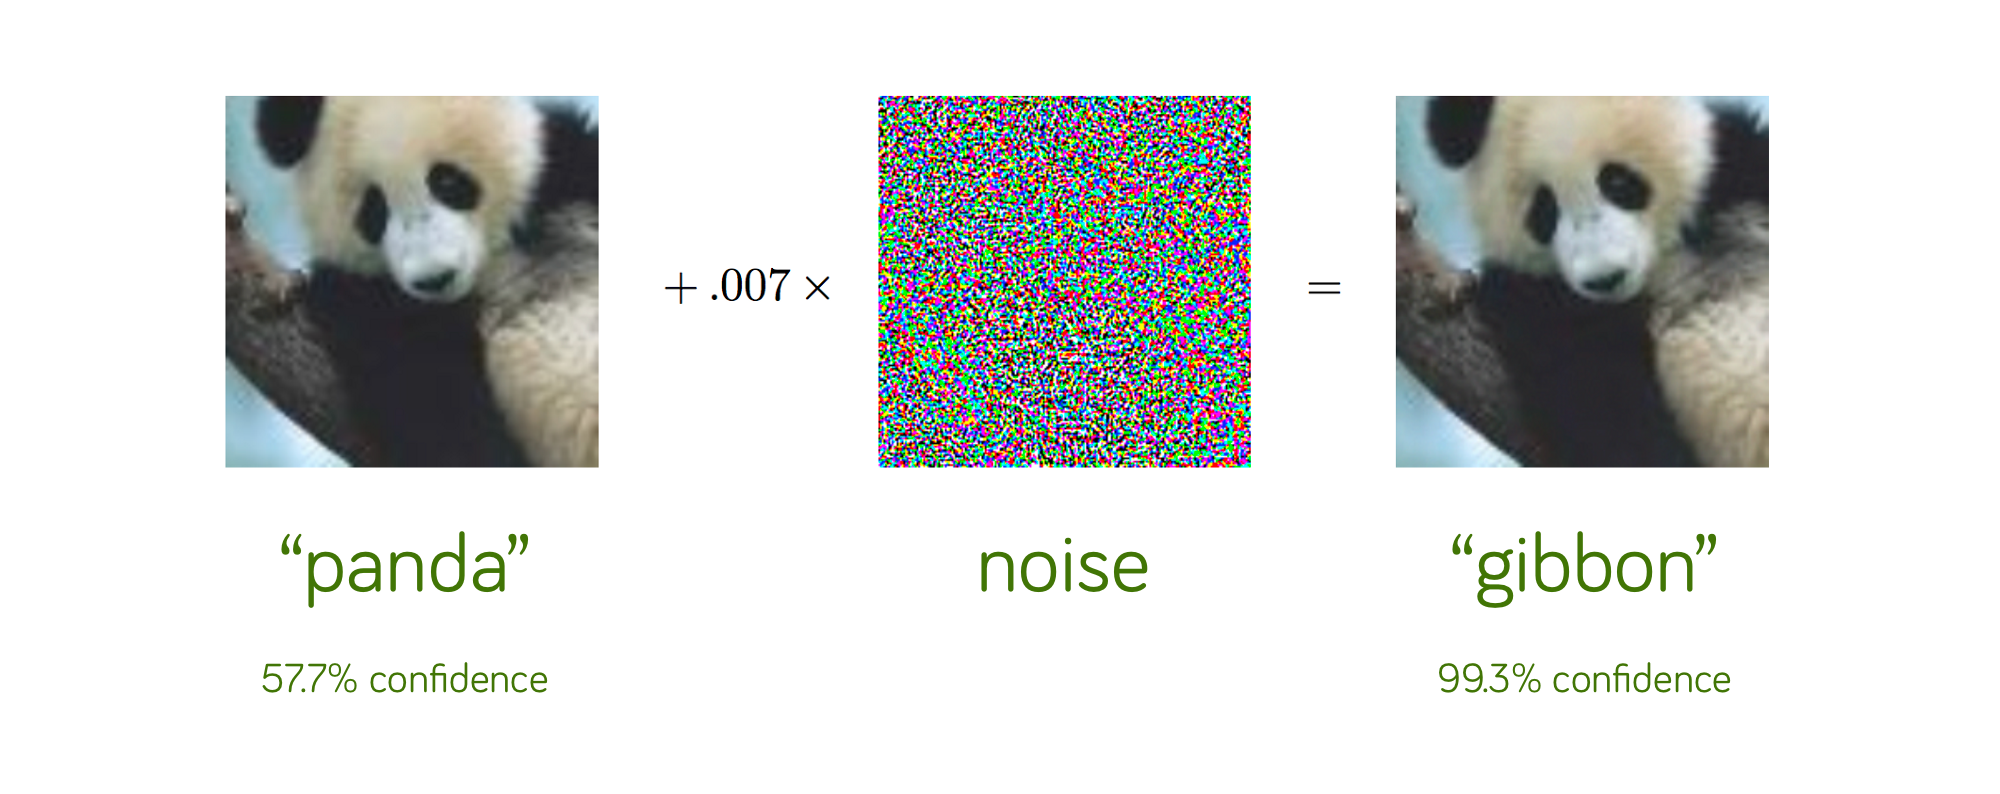
\includegraphics[width=0.8\linewidth]{images/panda_attack.png}
                \caption{An actual image of panda with a perturbation makes a novel deep neural network to misclassify as gibbon.}
                \label{fig:panda_attack}
            \end{figure}

        \item In 2017, another group demonstrated that it’s possible for these adversarial examples to generalize to the real world by showing that when printed out, an adversarially constructed image will continue to fool neural networks under different lighting and orientations. \Cref	{fig:example1} shows that an adversarial image  can be printed and any novel model will still misclassify it.
        
            \begin{figure}[htbp]
                \centering
                    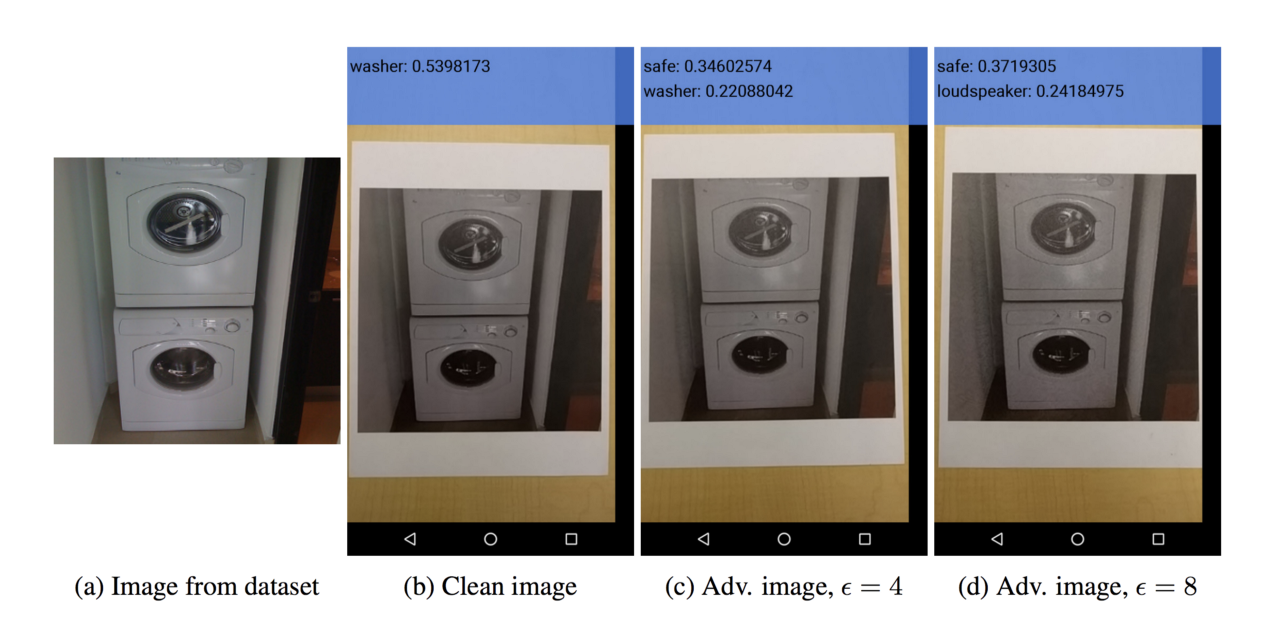
\includegraphics[width=0.7\linewidth]{images/example1.png}
                \caption{Printed adversarial image}
                \label{fig:example1}
            \end{figure}	
        \item Another interesting work, titled “Accessorize to a Crime: Real and Stealthy Attacks on State-of-the-Art Face Recognition” showed that one can fool facial recognition software by constructing adversarial glasses by dodging face detection altogether. The glasses in \cref{fig:example2} could let anyone impersonate someone else as well

            \begin{figure}[htbp]
                \centering
                    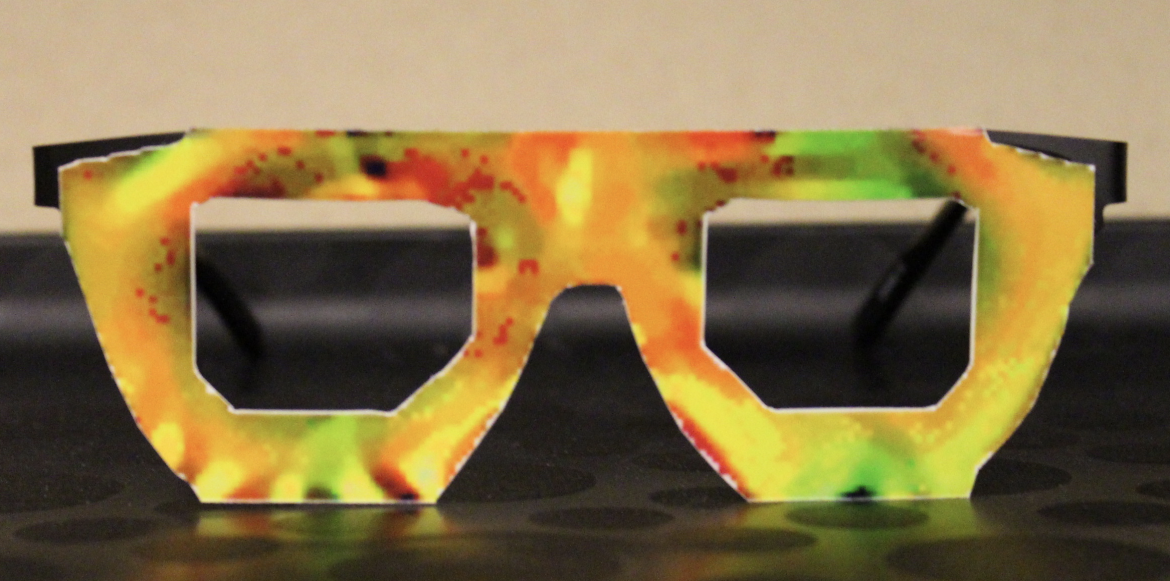
\includegraphics[width=0.4\linewidth]{images/example2.png}
                \caption{Adversarial glasses}
                \label{fig:example2}
            \end{figure}	
        
        \item Shortly after, another research group demonstrated various methods for constructing stop signs that can fool models by placing various stickers on a stop sign. The perturbations were designed to mimic graffiti, and thus “hide in the human psyche.” One of example is showcased in \cref{fig:example3}
        
            \begin{figure}[htbp]
                \centering
                    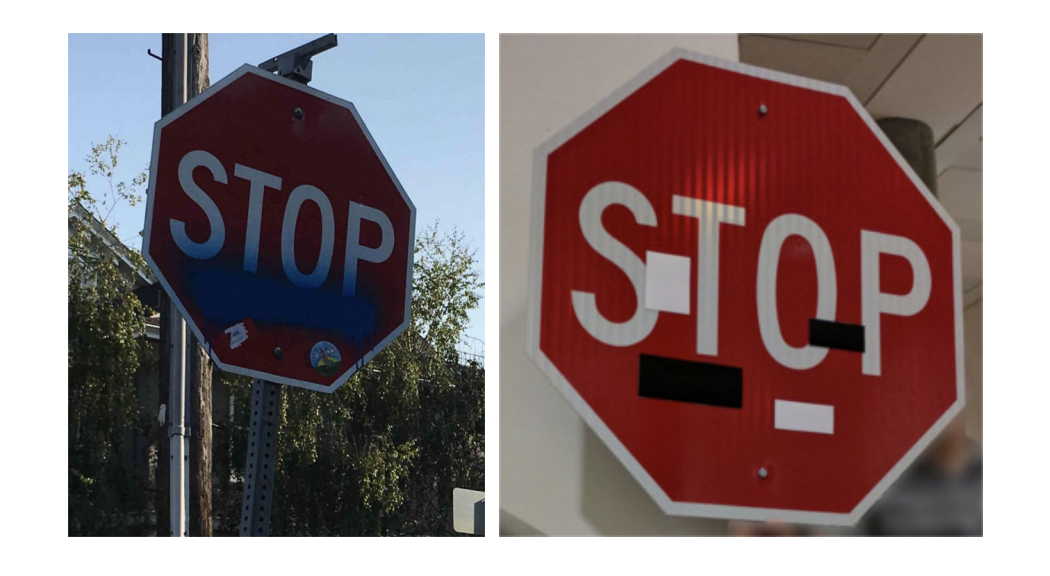
\includegraphics[width=0.4\linewidth]{images/example3.png}
                \caption{Adversarial attack by placing stickers on traffic sign boards}
                \label{fig:example3}
            \end{figure}	
        
        \item “Adversarial Patch”, a paper published at NIPS 2017 demonstrated how to generate a patch that can be placed anywhere within the field of view of the classifier and cause the classifier to output a targeted class. In their experiment, a banana is correctly classified as a banana. They then placed a sticker with a toaster printed on it which is still not enough to fool the network and it still continues to classify it as a banana. However, with a carefully constructed “adversarial patch” by them, they tricked the network into thinking that it’s a toaster. \Cref{fig:example4} represents their experiment. Anyone can download thier paper and print the patch for verification. To quote the authors, “this attack was significant because the attacker does not need to know what image they are attacking when constructing the attack. After generating an adversarial patch, the patch could be widely distributed across the Internet for other attackers to print out and use.”
        
            \begin{figure}[htbp]
                \centering
                    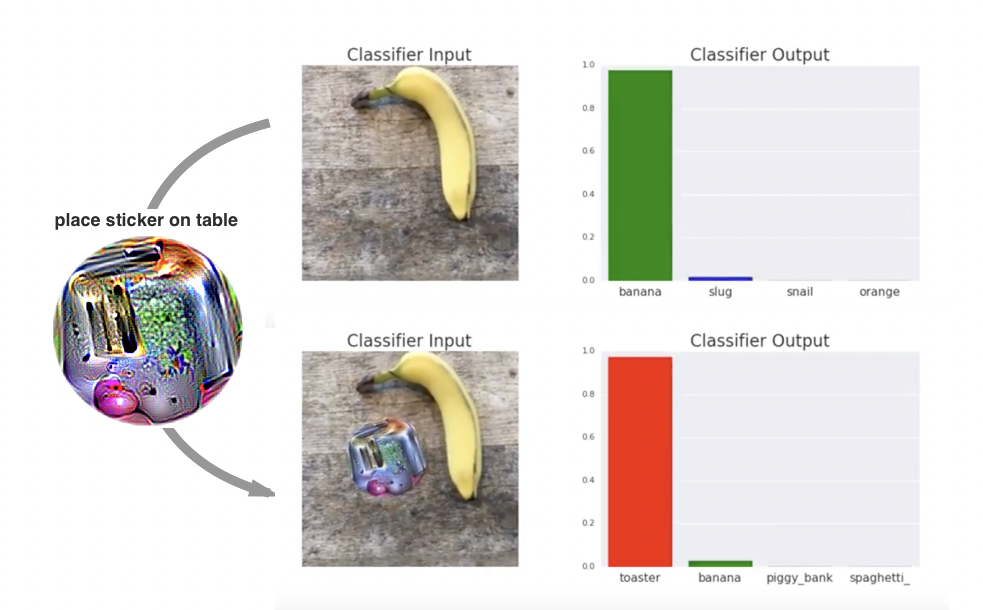
\includegraphics[width=0.7\linewidth]{images/example4.png}
                \caption{An actual image of panda with a perturbation makes a novel deep neural network to misclassify as gibbon.}
                \label{fig:example4}
            \end{figure}	
            
        \item Tesla, an automaker manufactures cars with autopilots. Their autopilots uses a very deep neural network to make decisions. They annualy organises an event and invites attackers to attack their system. Successful attackers gets a price money with gifts. Recently, some researchers performed adversial attack on their deep neural network and made their autopilot to change lane with incoming traffic. They have performed black-box attack. \Cref{fig:example5} give some intuition of the attack performed.
        
            \begin{figure}[htbp]
                \centering
                    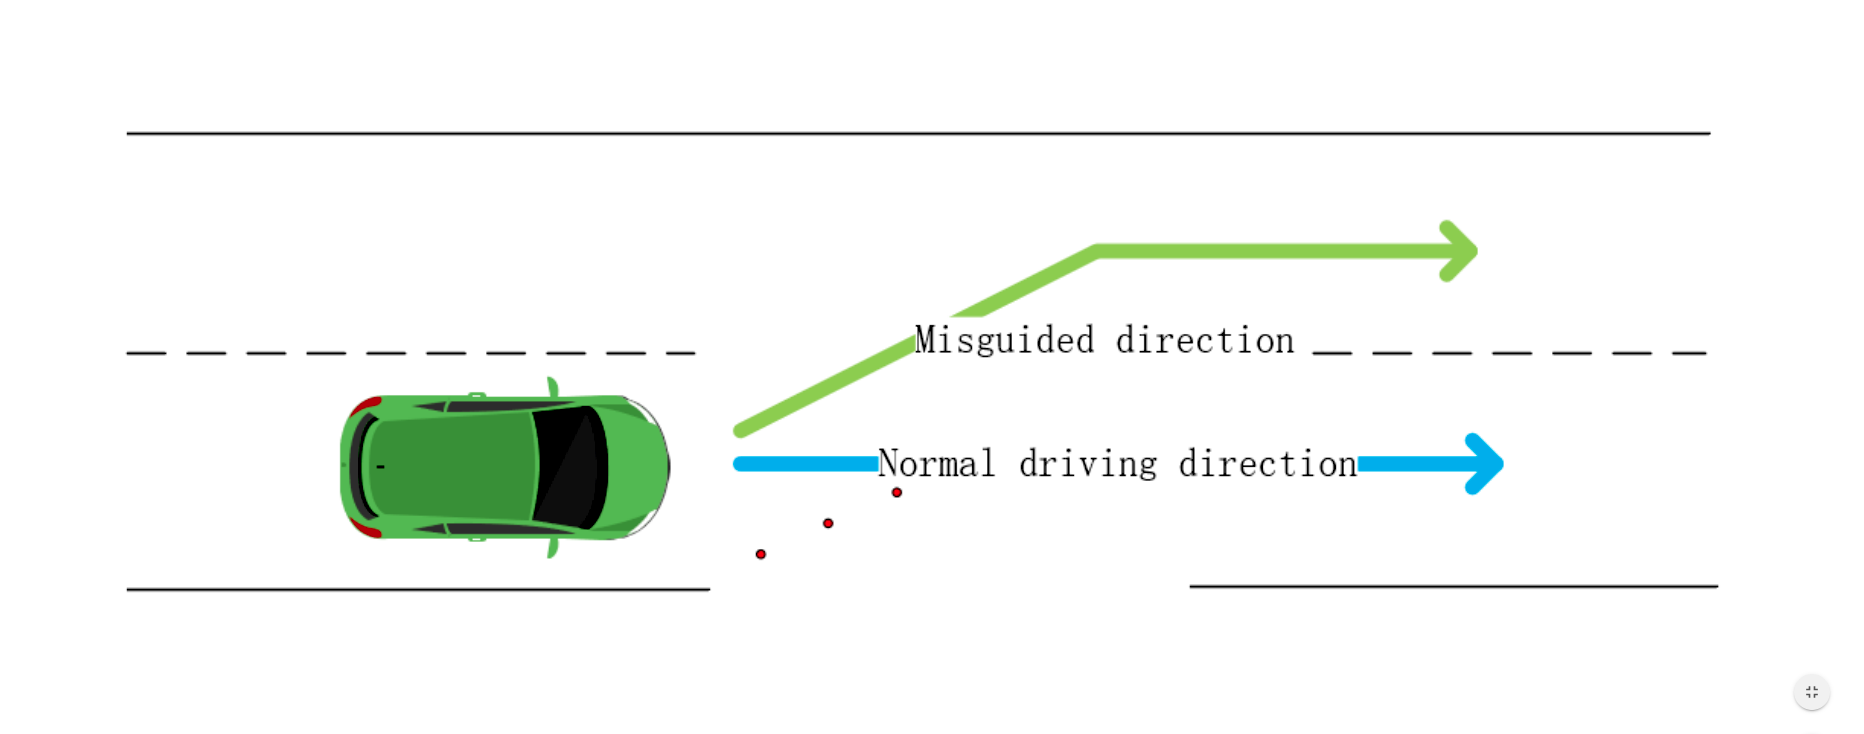
\includegraphics[width=\linewidth]{images/example5.png}
                \caption{An actual image of panda with a perturbation makes a novel deep neural network to misclassify as gibbon.}
                \label{fig:example5}
            \end{figure}
	\end{enumerate}
